%!TEX root =../MacbethThesis.tex
\acresetall
\chapter{Simulation of a Knowledge Commons with Presage2}

In this chapter we create a computer model of participatory sensing and use
this model to test our theory that by managing information and knowledge as a
commons, and according to Ostrom's principles for sustainable management of
common-pool resources we can improve the outcomes for agents in this system.

We first describe our model of participatory sensing, which approximates a
participatory sensing campaign as a reinforcement learning problem. This
approximation allows us to abstract the details of individual campaigns and
simply reason able where utility is accrued in the system. We then describe
the implementation of this system using the Presage2 platform, which we have
described in \autoref{ch:presage}. We then describe our implementation of the
provision and appropriation system outlined in \autoref{sec:iad} using the
Drools-EInst rule engine. We also describe the other institutional mechanisms
to manage the resource during the simulation. We give a description of how
agents play the reinforcement learning game and interact with the institution.
Finally, we describe the results of our experiments with this model.

\section{Modelling Participatory Sensing as a Reinforcement Learning Problem}

So far we have articulated participatory sensing as the contribution of
information by individuals to a pool. This collected information can then be
used to generate new derived information using some kind of knowledge.
However, we have yet to describe what this knowledge is.

In general, an algorithm which takes data as an input and gives information
about the data as an output can be classified as a \emph{machine learning}
algorithm. Data aggregation in participatory-sensing applications follows this
pattern. This learning may be \emph{supervised}, where data is labelled by an
expert and one aims to predict the value of the label given incomplete data,
or \emph{unsupervised}, where one looks for an underlying pattern in
unlabelled data.

Participatory sensing may deal with either of these types of machine learning.
Using raw sensor readings of, for example, temperature, and using them to
predict future temperatures would be \emph{unsupervised} learning from sensing
data. If these readings also had a user specified `comfort' level attached to
them, then we could use \emph{supervised} learning to work out if comfort
level is correlated with temperate and infer expected comfort levels from
temperature data.

When viewing participatory sensing as an agent-based system, we can see that
information is generated as a result of an action: that of taking a sensor
reading. This information, when combined with other information and processed
by a suitable machine learning algorithm, leads to derived information with
some additional value. In most cases, part of this value is offered back to
the original gatherer as an incentive to contribute. In many cases this
information improves a decision process in the agent, and the whole sensing
process can be seen as an optimisation feedback loop. Consider some of our
reviewed examples from \autoref{ch:kc}:

\begin{itemize}
\item Pothole Patrol~\citep{Eriksson2008}, VTrack~\citep{Thiagarajan2009}, Parknet~\citep{Mathur2010} and Waze all use information from participating cars to provide optimised route information back to them, such that they can reach their destination quicker, avoid hazards and so on.
\item With LiveCompare~\citep{Deng2009} users can derived reduce grocery costs from the information provided via the app.
\item Cloud2Bubble~\citep{Costa2012} gives feedback to users to improve their comfort levels during public transportation journeys.
\end{itemize}

These can be seen as reinforcement learning problems. Users are taking
repeated actions, such as driving, buying grocery items or taking public
transportation, and each time deriving both utility and information from the
process. This can be then used to optimise the process for the next iteration.
This process can be done individually, but participatory sensing can
significantly speed up this learning process.

Reinforcement learning is a form of machine learning where one aims to
determine which sequence of actions to take in order to maximise a cumulative
reward. This is a method of learning while interacting with the environment,
and based on the feedback given from each action. It differs from supervised
learning in that the agent is not provided with examples, it must learn
through trying actions. This reveals an important trade-off in reinforcement
learning, that of \emph{exploitation} vs. \emph{exploration}. This trade-off
is between exploiting a known good strategy and exploring unknown strategies
for one which may be better~\citep{Sutton1998}.

Participatory sensing is particularly useful for these kinds of problems as it
can reduce the need for exploration. In the case of vehicle navigation an
individual would have to do significant exploration to find a suitable route
in a new area. Expanding the number of vehicles contributing data allows
individuals to navigate new areas with little exploration required, and
therefore derive a better utility.

In most practical participatory-sensing applications, the aim is to infer the
utility of actions from the provided information and then provide advice on
the best action to perform next. For our model we simplify this process by
making the information provided the actual utility observed. This allows us
to frame a participatory sensing problem within the abstract reinforcement
learning framework, defined by \citet{Sutton1998}.

This framework, defines an \emph{agent} which interacts with an
\emph{environment} in discrete time-steps. Each time-step the agent receives
the environment's state and selects an action from the set of those available
from the current state. Then in the next time-step the agent receives a reward
from his action, and the new state and the process continues. The decision
about which action to take is done by the agent's \emph{policy}, and this is
what reinforcement learning aims to improve. The agent's goal is maximise its
total accrued reward.

We instantiate this framework with multiple agents in a shared environment.
Within this environment there are institutions available which provide
\emph{policies} via \emph{provision} and \emph{appropriation} actions. Instead
of generating actions themselves, with their own policy, agents provision
\emph{(state, action, reward)} tuples, and appropriate a suggested next action
from an institution. % TODO: figure

This model integrates the reinforcement learning framework with our framework
for participatory sensing as a provision and appropriation system from
\autoref{sec:iad}. The provision and appropriation actions from reinforcement
learning agents match those of \emph{gatherers} and \emph{consumers}.
\emph{Policies} are provided by \emph{analysts}. In our model we do not use
\emph{evaluators}, however they could be added to provide meta level analysis
of the quality of \emph{policies}, by determining the efficacy of actions
suggested by them.

% TODO: figure, prov and app system linked to game

% There are several issues when considering how to model a generic machine learning problem:
% \begin{itemize}
% \item How is information created? Usually through actions
% \item What is the value of a particular piece of information? What is the value of the incremental improvement given to the model?
% \item 
% \end{itemize}

\section{Model Implementation}

We now describe the implementation of this model of participatory sensing as an abstract reinforcement learning problem, using Presage2 and Drools-EInst. We firstly describe how the abstract reinforcement learning task is implemented on Presage2, and how specific tasks can be specified and used. We then integrate Drools-EInst to provide the institutional framework for the provision and appropriation system such that agents can interact with it. 

Our model implementation makes several assumptions about, and simplifications of, the participatory sensing problem we are modelling. Namely:

\begin{itemize}
\item The only flow of utility into the system is that generated by agents' actions on the reinforcement learning problem. For example an \emph{analyst} cannot sell information elsewhere to generate utility.
\item Utility is a trade-able currency. This reduces complexity by preventing the need for a separate currency.
\item Utility gained from an action is directly measurable by the agent.
\item Agents are working on the problem long-term, therefore we have repeated (inter)actions and thus can assume that agents are likely to be cooperative~\citep{Axelrod1984}.
\end{itemize}

The computer model is split into two independent components, which are then
linked by the agents' interaction with each component. These components are
the learning problem itself, and the electronic institution for participatory
sensing.

\subsection{Reinforcement Learning Problem}

The reinforcement learning problem is implemented directly using Presage2.
Actions submitted by agents are assessed according to the \emph{reward
function} of the environment and the agents' utility is updated accordingly.
Our implementation is generic, such that we can substitute in different reward
functions to test different scenarios without changing how agents play the
game. We outline this implementation here.

The reward function for a scenario is defined in terms of \texttt{State} and
\texttt{Strategy}\footnote{\emph{Action} from the reinforcement learning
framework is renamed to strategy to avoid conflict with the use of `action' as
a general term for both physical actions and the conventional ones used by the
institution}. The former represents the environment state for a given agent
(this state may be different for other agents in the same time-step), the
latter is a chosen action, or series of actions. This \texttt{Strategy} also
specifies if the agent wishes to measure the utility gained from the action.
This may come at a cost, which is an optional parameter to the game. If the
utility is to be measured the agent receives a \texttt{Measured} object, which
contains the $(\mathit{state}, \mathit{strategy}, \mathit{utility}, t)$ tuple
for this observation.

\emph{Policies} are defined by \texttt{Predictor}s. These select a strategy
given a current state and set of available strategies. The \texttt{Predictor}
can then be trained with \texttt{Measured} objects in order to learn the best
strategy choices. \texttt{Predictor}s implement general reinforcement 
learning algorithms such as Q-Learning and SARSA.

We can take the popular N-Armed Bandit problem from reinforcement learning to
specify a reward function. In this problem, agents can choose from $N$
actions, each of which have a different probability of paying out a reward.
There is no intermediate state in this game so the state is always empty, and
the \texttt{Predictor} simply aims to estimate the action with the highest
payout probability. These probabilities may also change over time, forcing the
\texttt{Predictor} to weight newer information higher than old.

Agents playing the N-Armed Bandit game are likely to experience varying
outcomes, largely due to the exploitation vs exploration trade-off.
Reinforcement learning policies often utilise probabilistic random exploration
of other strategies, leading to non-deterministic behaviour. From a modelling
perspective this increases the number of repeats required to achieve
statistically significant results.

Therefore, we aim to model the properties of a reinforcement learning policy,
while maintaining determinism. We utilise the results presented by
\citet[ch.2]{Sutton1998} that, when aggregated over multiple runs, using
Q-Learning on an N-Armed Bandit problem tends towards optimal action
selection. When plotting number of performed actions against chosen action
optimality this gives a logarithmic curve. Given this expected performance of
a policy, we define a reward function which, rather than depending on the
action itself, depends on the data in the policy used to select this action.

Given a \texttt{Predictor} trained with a set of \texttt{Measured} objects, $M$, we define the reward function for a given action at a time $t$, $r_t(a_t)$ as:
\begin{equation*}
r_t(a_t) = \sum_t^{t-W} \frac{|M_t|}{W*N}
\end{equation*}
Where $M_t$ is the subset of $M$ which were gathered at time $t$; $W$ is the time-window for which information is useful; and N is the maximum possible value of $|M_t|$.

This function returns a value between 0 and 1 which represents how good the
policy is. The size of the window-length parameter, $W$, adjusts the
function's sensitivity to keeping new information. Smaller values will reflect
problems with fast-changing strategies which need a constantly updated model,
while larger values model slower changing systems.

\subsection{Institution Design and Implementation}

We implement an electronic institution for the provision and appropriation of
information and knowledge, following the framework we outlined in
\autoref{sec:iad}, and using our rule engine for electronic institutions,
Drools-EInst. In these simulations we focus on addressing the first three of
Ostrom's principles in order to create an enduring, self-organising
institution. With these principles, and the requirements of participatory sensing as a provision and appropriation system, give the following tasks for the Institution:

\begin{itemize}
\item Clearly defined boundaries---The boundaries of the institution must be defined, not only who can contribute and withdraw resource units, but what resources are managed by the institution.
\item Provision and appropriation rules---Appropriate rules for the conditions. In this case the incentivisation of particular user roles to encourage contribution is important.
\item Collective-choice arrangements---That the rules can be modified by those who they affect.
\item Facility costs---
\end{itemize}

The Drools-EInst provision and appropriation system module provides the basis
of the resource pools in the institution. This is a role-based implementation
which allows the specification of multiple \texttt{Pool}s for different
resource types. The pool specifies which roles are permitted to contribute,
extract, and remove artifacts to/from the pool. This allows us to then build
institutionalised power for these actions, as shown in \autoref{lst:provapppow}.

\begin{drools}[label=lst:provapppow,caption={Institutionalised power for provision, appropration and removal from a pool of artifacts.}]
rule "Pow Provision"
	when
		RoleOf($a : actor, $r : role, $i : inst)
		Pool(inst == $i, contribRoles contains $r, $type : artifactMatcher)
	then
		insertLogical( new Pow($a, new Provision($a, $i, $type)));
end
rule "Pow Appropriate"
	when
		RoleOf($a : actor, $r : role, $i : inst)
		Pool(inst == $i, extractRoles contains $r, $type : artifactMatcher)
	then
		insertLogical( new Pow($a, new Appropriate($a, $i, $type)));
end
rule "Pow Remove"
	when
		RoleOf($a : actor, $r : role, $i : inst)
		Pool(inst == $i, removalRoles contains $r, $type : artifactMatcher)
	then
		insertLogical( new Pow($a, new Remove($a, $i, $type)));
end
\end{drools}

Successful provisions are added to the set of artifacts stored in the pool. As
artifacts are heterogeneous agents need to be able to specify an artifact when
appropriating. This is done through a \texttt{Request} which searches for
artifacts in the pool matching a query. The individual artifacts can then be
appropriated. The same process applies to \texttt{Prune} actions for artifact
removal.

The running of the institution isn't free, however. We implement
\emph{facility} costs using four parameters:

\begin{itemize}
\item Sunk costs---This cost is a one-off cost incurred when the institution is created. This reflects initial hardware/software purchase etc.
\item Fixed costs---This is a recurring cost each time-step. This would reflect long-term lease of equipment etc.
\item Marginal storage costs---This is a recurring cost proportional to the number of artifacts in the pool. For example renting storage space in a cloud data-centre.
\item Marginal transaction costs---This is a recurring cost proportional to the number of provision/appropriation requests in the last time-step. This reflects the cost of processing power or bandwidth in a cloud computing environment.
\end{itemize}

These costs are calculated and the institution invoiced each time-step. If the
institution is no longer able to pay these invoices it goes bankrupt, and will
cease to operate.

% sub fee + pay for provision/appropriation  

In order to pay for facility costs the institution provides two mechanisms.
The first is a simple cost sharing, there certain nominated roles share the
cost of the outstanding institution invoices. This shares costs equally and
ensures that, provided the agents can afford it, the institution's costs are
covered. The other method is the use of a subscription fee on a per role
basis. This fee charges per time-step for the occupation of a role. The rules
to implement both of these methods are shown in \autoref{lst:instcosts}. These
rules calculate a total value due per agent and then create an obligation to
\texttt{Transfer} the required amount. It is then up the agent itself whether
it fulfils the obligation.

\begin{drools}[label=lst:instcosts,caption={[Paying for institution costs.]Paying for institution costs. Under cost sharing, the rule generates the set of paying agents from the specified \texttt{payRoles} of the institution and the \texttt{RoleOf} facts designating current roles. The amount required to pay off the institution's negative balance is split between these agents. \texttt{PaidInstCosts} is a control fact used to ensure that this rule only triggers once per institution per time-step.\\ The subscription fee rules uses a \texttt{subscriptionFee} fluent in the institution to select each agent in turn and issue a fee based on the current fee value. \texttt{FeeIssued} is a control fact to ensure the rule can only trigger once per agent per institution per time-step.}]
rule "Share institution costs"
	when
		$i : DataInstitution($r : payRoles)
		$acc : Account(holder == $i, balance < 0, $bal : balance)
		T($t : t)
		not( PaidInstCosts($i, $t;) )
		accumulate( 
			RoleOf(inst == $i, $r contains role, $a : actor); 
			$payers : collectSet($a);
			$payers.size() > 0)
	then
		double balanceDue = -1 * $bal / $payers.size();
		for(Object o : $payers) {
			Actor a = (Actor) o;
			insert( new Obl(a, new Transfer(a, $i, $i, balanceDue) ));
		}
		insert( new PaidInstCosts($i,$t) );
end
rule "Institution Subscription Fee"
	when
		RoleOf($a : actor, $i : inst, $r : role)
		DataInstitution(this == $i, subscriptionFees.containsKey($r), $fees : subscriptionFees)
		T($t : t)
		not( FeeIssued($a, $i, $t;) )
	then
		insert( new FeeIssued($a, $i, $t) );
		double fee = $fees.get($r));
		if(fee > 0) {
			insert( new Obl($a, new Transfer($a, $i, $i, fee) ) );
		}
end
\end{drools}

In order to incentivise provision of useful artifacts to the institution we
offer a mechanism for remuneration of providers. This can be done either
through a payment on provision of an artifact, or when a provisioned artifact
is appropriated. While the former places a uniform value on each artifact, the
latter allows greater remuneration for more valuable or useful artifacts.
Furthermore, the latter payments can be funded by the institution easier, by
simply charging the fee directly to appropriators. The implementation of the
pay on appropriation method is shown in \autoref{lst:apppay}.

\begin{drools}[label=lst:apppay,caption={[Drools specification of payment for provision of artifacts]Drools specification of payment for provision of artifacts. The first rule identifies an appropriation, the original provision action for the appropriate resource, and checks that both agents are still occupying roles in the institution. The provider is then paid the specified provision reward. \texttt{FeeIssued} is a control fact to prevent duplicate payment.\\ The second rule counts the number of appropriations from a pool by each agent in a single time-step. In then issues an oligation to pay the specified fee for each of these appropriations.}]
rule "Pay provider on appropriation"
	when
		T($t : t)
		$app : Appropriate(t == $t, $art : artifact, $i : inst, $appropriator : actor, valid == true)
		MeteredPool(inst == $i, payOnAppropriation > 0, artifacts contains $art, $pay : payOnAppropriation)
		Provision($provider : actor, inst == $i, artifact == $art, actor != $appropriator, valid == true)
		RoleOf(inst == $i, actor == $appropriator ) // appropriator has a role
		RoleOf(inst == $i, actor == $provider ) // provider has a role
		not( FeeIssued( $appropriator, $app, $t ;) )
	then
		insert( new Transfer($i, $provider, $pay, $t) );
		insert( new FeeIssued($appropriator, $app, $t) );
end
rule "Pool appropriation fee"
	when
		RoleOf($a : actor, $i : inst, $r : role)
		$p : MeteredPool(inst == $i, appropriationFees.containsKey($r), $matcher : artifactMatcher, $fees : appropriationFees)
		T($t : t)
		not( FeeIssued($a, $p, $t;) )
		accumulate( Appropriate($item : artifact, actor == $a, inst == $i, t == $t, $matcher.matches($item));
			$count : count($item); $count > 0)
	then
		double fee = $fees.get($r)
		if(fee > 0) {
			insert( new Obl($a, new Transfer($a, $i, $i, fee * $count) ) );
		}
		insert( new FeeIssued($a, $p, $t) );
end
\end{drools}

% voting

We implement collective choice using the Drools-EInst voting module. This
provides configurable voting for any issue. An \texttt{Issue} specifies
something which can be voted on, and how the voting is done in terms of:

\begin{itemize}
\item which agent roles are empowered to open and close a ballot on the issue,
\item which agent roles are empowered to vote in a ballot on the issue,
\item how votes should be cast (e.g.\ single choice, preference list, rank order),
\item what the valid choices are,
\item how the winner is determined from the set of votes (e.g.\ plurality, borda count etc.)
\end{itemize}

The module provides the institutionalised powers based on this specification,
and rules to process agent actions to open ballots, vote, and declare winners.
\autoref{lst:voterules} shows examples of the implementation of these rules.

\begin{drools}[label=lst:voterules,caption={Opening of ballots and voting.}]
rule "Open Ballot"
	when
		$open : OpenBallot($a : actor, $i : inst, $is : issue, $t: t, valid == false)
		Issue(this == $is)
		Pow(actor == $a, this.matches($open))
	then
		insert( new Ballot($is, $t) );
		modify($open) {
			setValid(true);
		}
end
rule "Pow open ballot"
	when
		$is : Issue($i : inst, $r : cfvRoles)
		RoleOf($h : actor, inst == $i, $r contains role)
		not( Ballot(issue == $is, status == Ballot.Status.OPEN) )
	then
		insertLogical( new Pow($h, new OpenBallot($h, $i, $is) ) );
end
rule "Pow Vote"
	when
		$b : Ballot(status == Ballot.Status.OPEN, $r : voteRoles, $t : started)
		RoleOf($a : actor, inst == $b.issue.inst, $r contains role)
		not( Vote(actor == $a, inst == $b.issue.inst, ballot == $b, t > $t, valid == true) )
	then
		insertLogical( new Pow($a, new Vote($a, $b.getIssue().getInst(), $b, null) ) );
end
\end{drools}

Using this module collective choice can be simply implemented by first,
specifying an \texttt{Issue} to apply voting to, and then secondly, writing a
rule to react to the appropriate winner declaration and update fluents to
reflect the consequence of the vote.

For example, to implement a dynamic subscription fee for an institution we
create a \texttt{SubscriptionFee} which extends \texttt{Issue}. This issue
implements a function \texttt{updateFee} which we can use to update the fee
following a vote. This process can then be implemented in a simple rule:

\begin{droolsinline}
rule "Change Subscription fees"
	when
		$issue : SubscriptionFee($i : inst)
		Declare( ballot.issue == $issue, $w : winner, valid == true )
	then
		$issue.updateFee($w);
end
\end{droolsinline}

We use this method to implement collective choice for institution subscription
fees and pool appropriation fees.

% Pool/inst instantiation

This implementation brings together the general purpose tools from Drools-
EInst, with the library of general purpose modules to create an implementation
of generic components for a provision and appropriation system. For the
specific simulation we wish to simulate we construct an instance we the
correct components enabled and configured. This is done by simply inserting
the configured facts into the rule engine, loaded with the general
specification.

For our reinforcement learning problem we require two pools, one for
\texttt{Measured} information, and another for \texttt{Predictor}s for action
selection. The former allows contributions from \emph{gatherers}, extraction
by \emph{analysts} and removal from a \emph{manager} role. For the latter pool
contribution and extraction roles are reversed. These pools can also be
configured with initial provision or appropriation fees and collective choice
regarding how these can be changed.

\subsection{Agent Implementation}



\section{Evaluative Criteria}

In our analysis of participatory sensing using the \ac{IAD} framework, we finished by
discussing five evaluative criteria which can be used to assess the efficacy
of a knowledge commons. We revisit these within the context of our model to
obtain quantitative measures of system performance. We can then use these as
tools for objective comparison of difference approaches to managing
information and knowledge resources.

\begin{enumerate}
\item \emph{Increase in knowledge} evaluates the extent to which the system has
generated new knowledge. In our model, utility gained is a direct measure of the
quality of knowledge. Therefore, we can give a metric of the knowledge generated
by the system as the sum of all agent utilities.

\begin{equation}
\mathit{knowledge} = \sum^{a\in A} u
\end{equation}

\item \emph{Sustainability} measures whether a system endures in the the long term.
This can be simply measured by testing whether the institution has not shut down 
due to bankruptcy after a fixed period of time.

\begin{equation}
\mathit{endures} = \mathit{account}(i) > 0
\end{equation}

\item \emph{Participation standards} measures the level of participation within the 
institution. As our agents are implemented such that they will resign roles they 
no longer need, the number of occupied roles is a good measure of participation.

\item \emph{Efficiency} determines the economic cost of the system relative to its productive output. In this case the cost is purely measured by facility cost and the output is the increase in knowledge.

\item \emph{Equity.} Given that all agents have the potential to achieve the same, we can expect that an equitable system will result in all agents achieving the same utility. Therefore the equity can be measured as the standard deviation of all agents' final utilities. 
\end{enumerate}

\begin{figure}
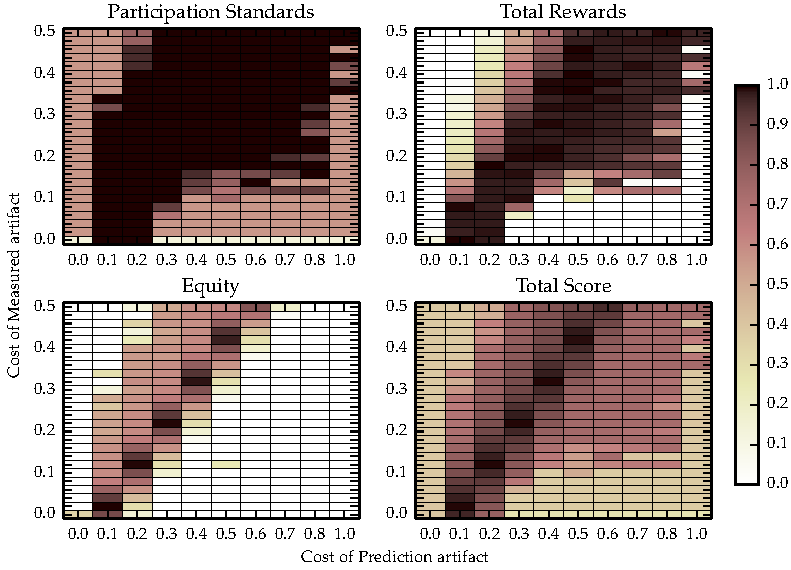
\includegraphics{gfx/kc/static_0.pdf} 
\caption{No measuring cost.}
\end{figure}

\begin{figure}
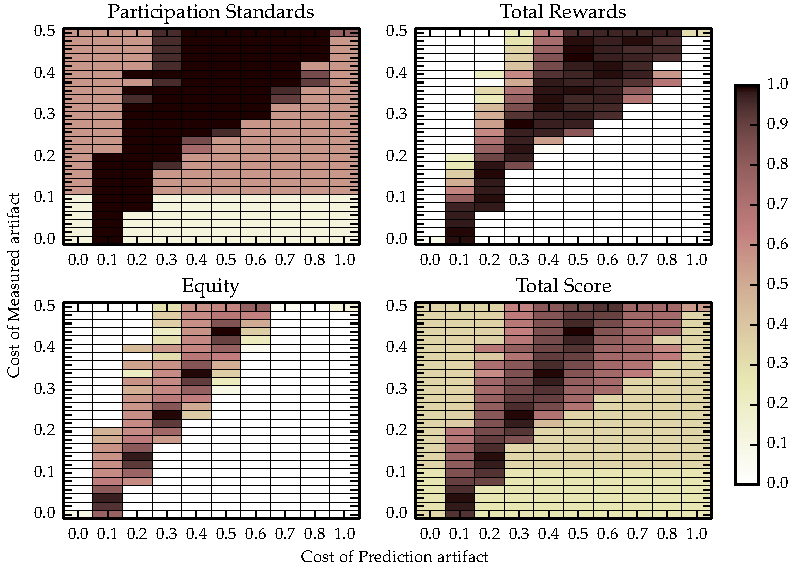
\includegraphics{gfx/kc/static_1.pdf} 
\caption{Measuring cost = 0.1.}
\end{figure}

\begin{figure}
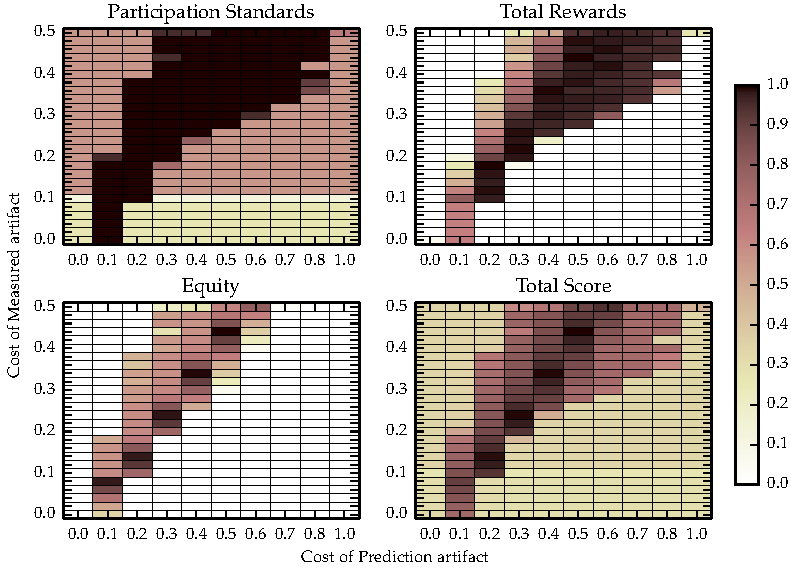
\includegraphics{gfx/kc/static_1_3nc.pdf} 
\caption{3 NC.}
\end{figure}

\begin{figure}
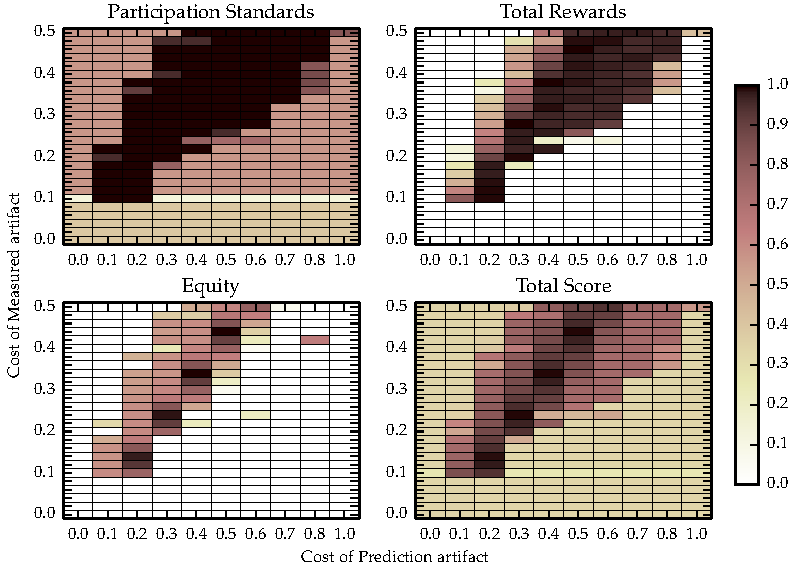
\includegraphics{gfx/kc/static_1_6nc.pdf} 
\caption{6 NC.}
\end{figure}

\section{Simulation Setup}

We model a participatory sensing problem as a reinforcement learning problem (See Sutton \& Barto). Policies are knowledge artifacts, which can be appropriated and used to chose actions. Agents are able to measure directly the reward from an action when performing it. Their aim is to maximise rewards over time by training a better policy. All agents play the same game, so policies and measurements are useful for everyone, and one agent's measurements can be used to train another's policy.

As policies will improve with more information, the best strategy for agents will be to pool their information and knowledge together. 
Therefore, by forming an institution around this information and knowledge, everyone should be able to achieve a better utility overall.

%The simulation is set up as a symmetric participatory sensing problem. This is a problem where agents are playing a repeated game where, in each round, a strategy played by the agent yields a reward. Agents are able to measure their previous rewards. They aim to maximise their reward over time by learning the best strategy to choose. As all agents are playing the same game this learning can obviously be improved by gathering together this information. Additionally not all agents will have the knowledge or capability to do this learning themselves. 

The institution is constructed as a provision and appropriation system with two pools. One for information as gathered by the learning agents, and the other for knowledge provided by analysts. This problem is symmetric as each group of agents will provision to one pool and appropriate from the other---learning agents provision information and appropriate knowledge and appropriate information and provide knowledge---thus they are also dependant on each other. If the institution is unsatisfactory for one group and they leave it will quickly become unsatisfactory for the others too.

The utility generated from the learning problem acts as the only external input of value into the system, while paying for facility costs is the only way of value flowing out of the system. All other transactions are endogenous. There is also a possibility, as seen in many real-world participatory sensing systems, of other exogenous rewards from ownership of a data-set, however we do not simulate this.

\subsection{Rewarding Knowledge}

In order to model the additive value of information when combined for learning we use an artificial reward function which gives a utility proportional to the quality of policy used to chose an action. The quality of a policy is defined as the number of information samples over a time window from the current time:

A policy is a tuple containing a set of data samples: $P = <S>$. A predictor can recommend an action for an agent: $\mathit{selectAction}(P,t) \rightarrow s_t$. Using this action then yields a reward: $u(s_t) = \sum_t^{t-W} \frac{|S_t|}{W*N}$ where $W$ is a time-window size for which information is useful and $N$ is maximum number of samples possible in one time-step. This function returns a value between 0 and 1.

\subsection{Agent strategies}

\begin{itemize}
\item Sustainable
\item Profitable
\item Greedy
\end{itemize}

\section{Experiments}

\subsection{The Problem of Supply}\label{sec:supply}

This first set of experiments looks at the problem of provisioning an institution for the problem we have outlined. Despite having a simple game where we can seemingly trivially generate utility, getting together disparate agents to all contribute and keeping it sustainable over the long time requires negotiating several hurdles. 

We will see these hurdles as we follow the process of building a centralised institution for this problem. This institution has a single agent who acts as a manager for the institution and as complete control over institutional fluents.

The experimental setup is as follows:
\begin{itemize}
\item One institution with information and knowledge pools.
\item 10 gatherer/consumer agents who are members of the institution.
\item One analyst agent providing knowledge for the institution.
\item One initiator agent managing the institution.
\item One independent agent as a control benchmark. This agent has the same knowledge as the analyst, but only uses self-gathered information.
\end{itemize}

\subsubsection{Facility Cost}

Storing information and knowledge, and other infrastructure required for the institution will incur facility costs. We have two profiles to model facility costs:
\begin{itemize}
\item High sunk cost --- A high initial sunk cost (for infrastructure acquisition), followed by a lower fixed cost each time-step ($\mathtt{sunk\_cost}=50$, $\mathtt{fixed\_cost}=1$).
\item High fixed cost --- No initial sunk cost, higher fixed cost ($\mathtt{sunk\_cost}=0$, $\mathtt{fixed\_cost}=2$).
\end{itemize}

We are running simulations over 200 time-steps, so these profiles would correspond to a total incurred cost of 250 and 400 respectively.

\begin{figure}
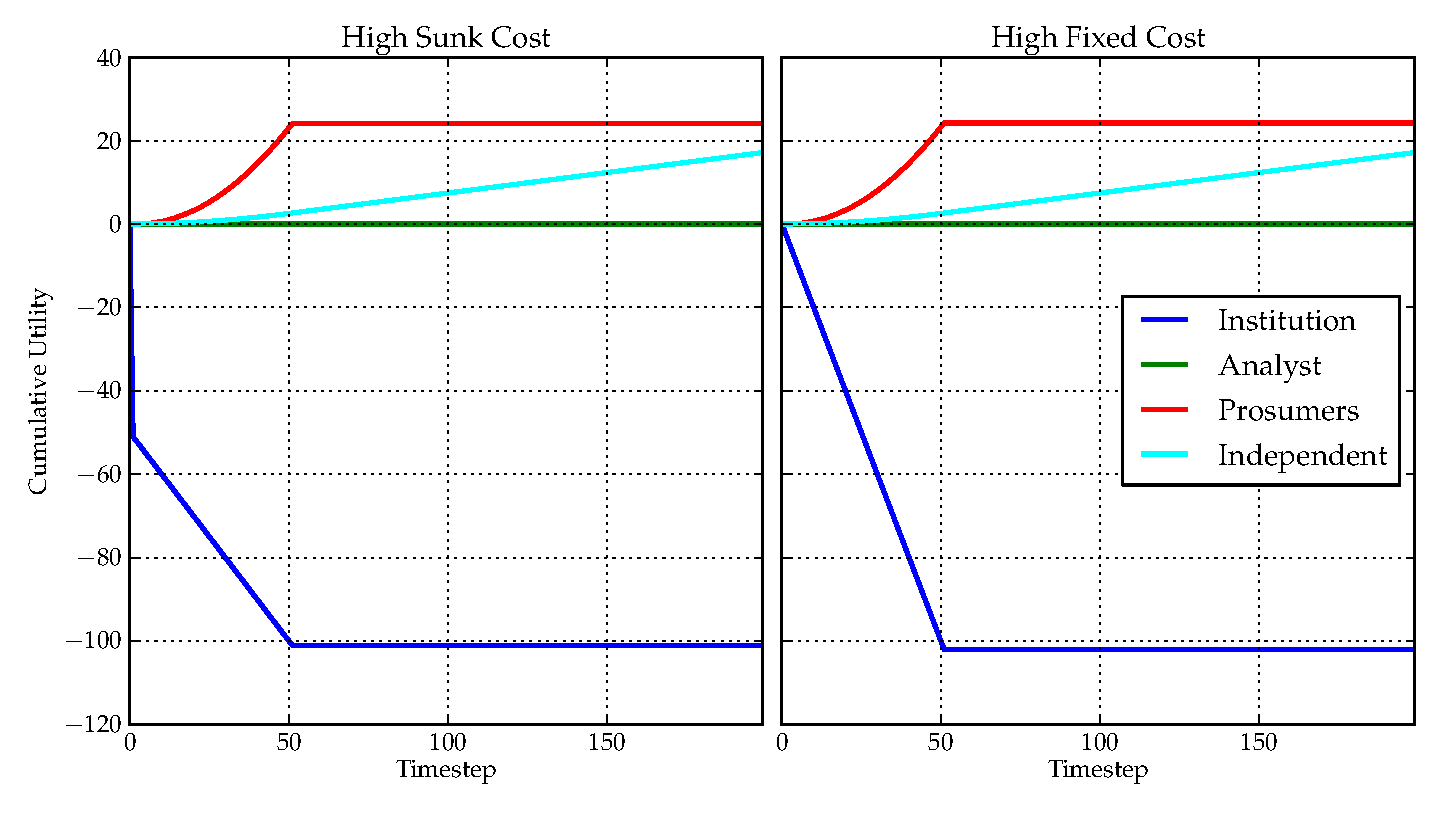
\includegraphics[width=\linewidth]{gfx/kc/facility1v2.pdf} 
\caption{Cumulative agent utilities over time in basic centralised institution with high--sunk and high--fixed facility profiles.}\label{fig:facility1}
\end{figure}

Figure~\ref{fig:facility1} shows the utilities in this scenario. In both cases the institution runs out of resources to pay for facilities after 50 timesteps, at which point the institution ceases to function. As the in-flow of utility into the system (to prosumers) is separate from where the facility is paid for (by the initiator) then the system cannot endure without the charity of the initiator. Therefore without exogenous income for this agent we require a way for prosumers to contribute to the facility costs.

One method we can use is to have a subscription fee. This is a payment to the institution each timestep which one is occupying a certain role. The level of this fee is determined by the initiator who has the sole power to set its value. 

\begin{figure}
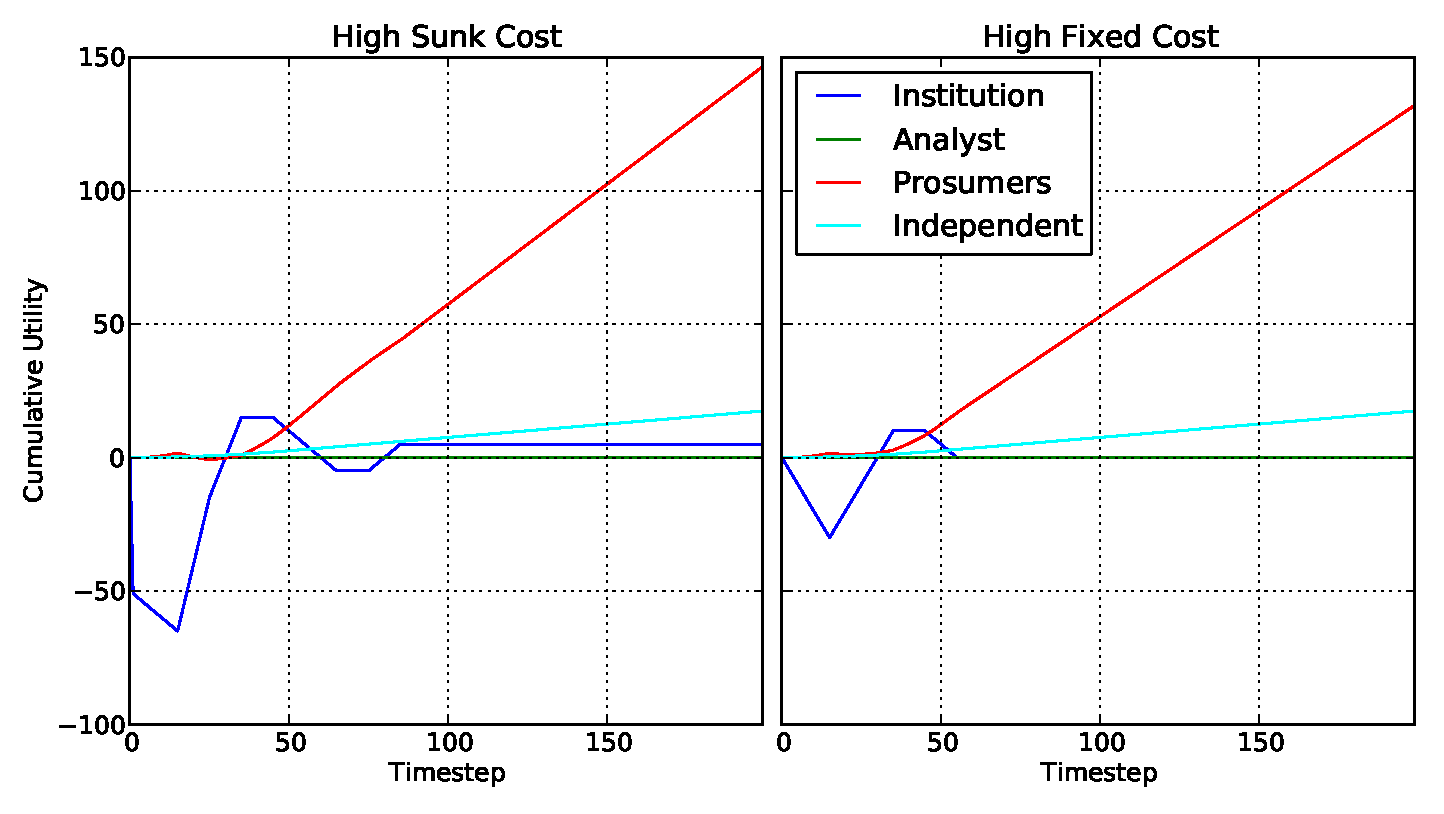
\includegraphics[width=\linewidth]{gfx/kc/facility2.pdf} 
\caption{Cumulative agent utilities over time in centralised institution using subscription fees with high--sunk and high--fixed facility profiles.}\label{fig:facility2}
\end{figure}

Figure~\ref{fig:facility2} shows agent utilities once subscription fees are introduced. The rate dynamically adjusts to ensure that the institution breaks even and that the institution endures. Here we also see the benefit of the institution. Prosumer agents accrue over 7.5 times more than the independent control agent in each case due to having 10 times more data and only small additional overheads.

\subsubsection{Compensating Analysts}

Figures~\ref{fig:facility1}~\&~\ref{fig:facility2} from the previous section both show zero utility gained for the analyst agent. However are having to appropriate information and process it in order to generate the knowledge which they provision. Given that this knowledge enables a large increase in reward for the prosumer agents, analysts may expect some remuneration.

This can be achieved by paying an analyst when knowledge is appropriated. Again the initiator can set the rate for this payment. Table~\ref{tab:analyst1} shows final utilities for agents when a fixed rate of 0.1 per appropriation is set.

\begin{table}
\centering
\begin{tabular}{c|c||c|c}
Facility Profile & Pay Analysts? & Prosumers & Analyst \\ 
\hline \hline
High sunk & no & 142 & 0 \\ 
\hline 
High sunk & yes & 127 & 157 \\ 
\hline 
High fixed & no & 128 & 0 \\ 
\hline 
High fixed & yes & 112 & 144 \\ 
\end{tabular}
\caption{Compensation of analysts}\label{tab:analyst1}
\end{table} 

\subsubsection{Compensating Gatherers}

In the previous examples all prosumers always gather information, and always provision it, as there is no cost for them in this process. However in some cases there is likely to be some costs associated with gathering information. In turn this may cause some agents to `free-ride' by not gathering or provisioning information while still receiving the benefits of the institution. Again we can simply introduce a payment for provision or appropriation of this information.

\begin{table}
\centering
\begin{tabular}{c|c|c||c|c|c}
Facility Profile & Pay Gatherers? & No. Greedy & Compliant & Non-compliant & Analyst \\ 
\hline \hline
High sunk & no & 2 & 74 & 93 & 157 \\ 
\hline 
High sunk & no & 5 & -8 & -1 & -8 \\ 
\hline
High sunk & yes & 2 & 91 & 92 & -4 \\ 
\hline 
High sunk & yes & 5 & 92 & 91 & -4 \\ 
\hline  
High fixed & no & 2 & 61 & 81 & 144 \\ 
\hline 
High fixed & no & 5 & -8 & -10 & -2.5 \\ 
\hline
High fixed & yes & 2 & 67 & 64 & -4 \\ 
\hline 
High fixed & yes & 5 & 64 & 68 & -4 \\ 
\end{tabular}
\caption{Compensation of gatherers with measuring cost of 0.1}\label{tab:gatherers1}
\end{table} 

Table~\ref{tab:gatherers1} shows cumulative utility for compliant and non-compliant prosumers, and analysts when a measuring cost is introduced. Non-compliant prosumers will not generate information to provision if it is not profitable to do so (payment for provision less than measuring cost). The data shows that introducing a payment to gatherers reduces this non-compliant behaviour. However the knock-on effect is that it is more expensive for the analyst to operate, and in fact this agent cannot afford to appropriate all of the available information as before. This results in lower quality knowledge and less total utility generated by the system.

This problem can be prevented by simply increasing the pay to the analyst for appropriations. Figure~\ref{fig:measuringCost} shows the average cumulative utilities for each agent group with three institution configurations:
\begin{enumerate}
\item Without payment to gatherers.
\item With payment to gatherers.
\item With payment to gatherers and increased payment to analyst.
\end{enumerate}
Each configuration is tested with two and five non-compliant prosumers out of the ten total.

\begin{figure}
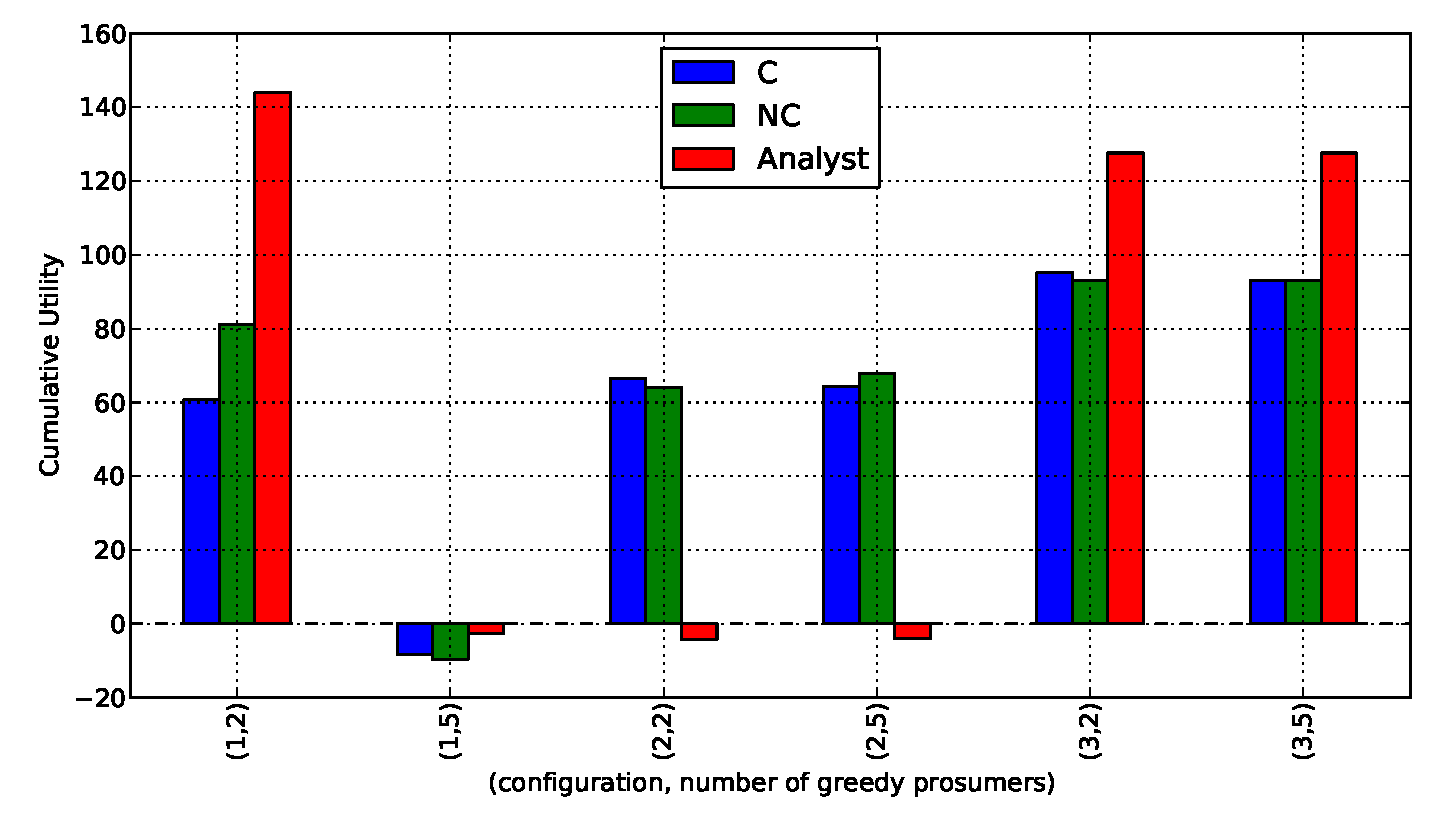
\includegraphics[width=\linewidth]{gfx/kc/measuringCost1.pdf} 
\caption{Average cumulative utilities for Compliant prosumer (C), Non-compliant prosumer (N) and Analyst groups under three institution configurations and with 2 and 5 N agents.}\label{fig:measuringCost}
\end{figure}

From the graph we can see that properly compensating the analyst allows for better knowledge to be generated.

\subsection{Self-Organisation}

We have seen in the previous section that we require several mechanisms in place to create an effective institution. Using static examples allows us to test certain situations, however for long-term robustness we require that these fluents, such as subscription fees, and provision and appropriate fees, can be changed over time to react to external and internal conditions. We also require that the agents in the system can do this themselves, without external supervision, so that the system is self-organised.

We do this by allowing these fluents to be changed by vote. Periodically agents are permitted to vote on the value of a fluent, and if the vote is decisive, the value is changed. With this method we can define three models of institutional governance:
\begin{itemize}
\item Centralised --- A single agent has the power to vote on all issues.
\item Market --- Those who provision an artifact (i.e. supply) have the power to vote on its price.
\item Principled --- Following Ostrom's third principle, those affected by an operational rule are permitted to vote on it: Anyone with provision or appropriation rights to a pool can vote on its fees.
\end{itemize}

\subsection{Centralised}

With centralised governance the initiator agent has control over subscription, gatherer pay, and analyst pay rates. Figure~\ref{fig:centralised1} shows a combination of:
\begin{itemize}
\item Setting subscription rates to cover facility costs.
\item Setting a fair appropriation fee to compensate analysts.
\item Setting a reward for provisions when there is a measuring costs to incentivise provisions.
\end{itemize}

\begin{figure}
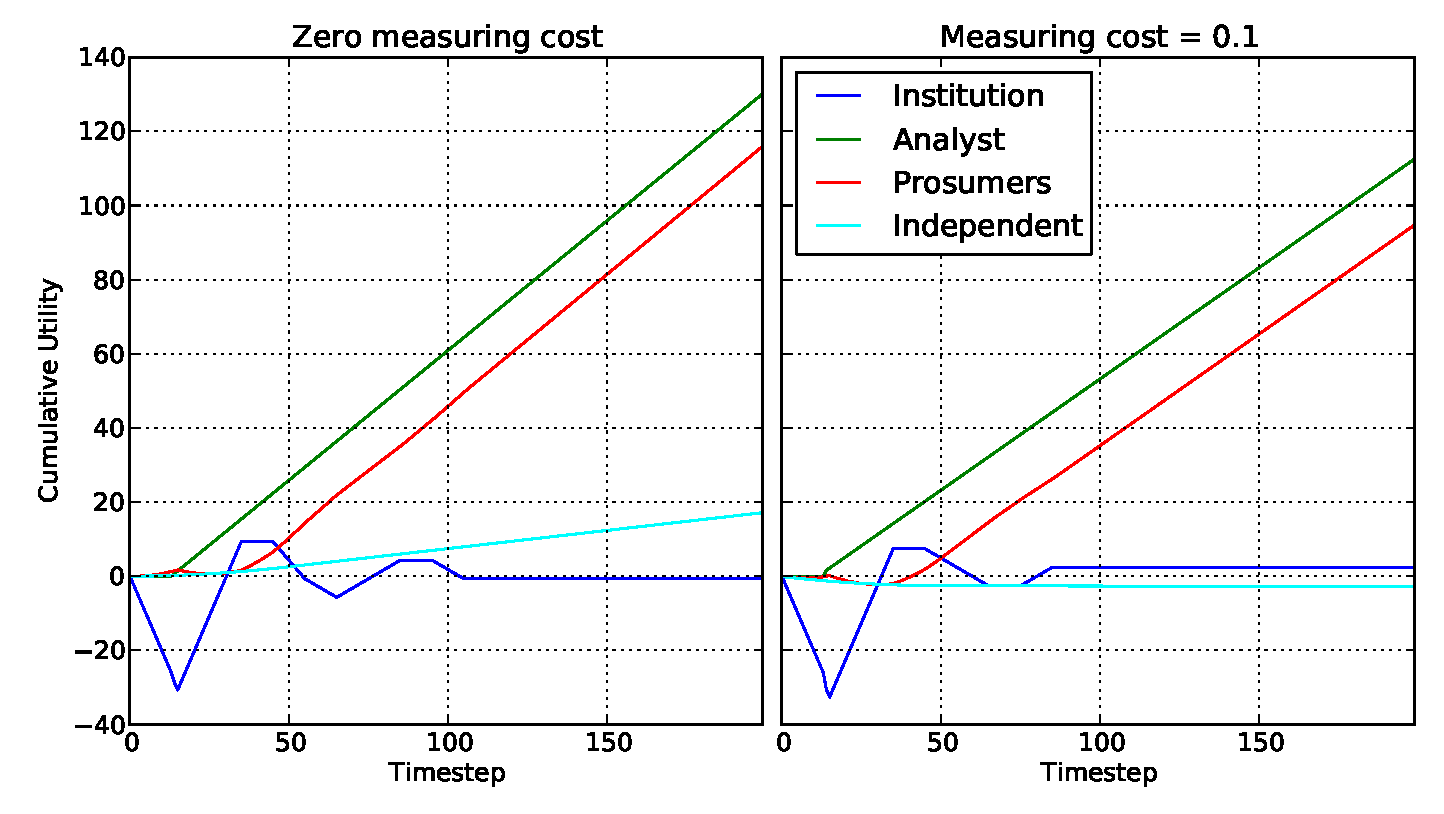
\includegraphics[width=\linewidth]{gfx/kc/centralised1.pdf} 
\caption{Cumulative utility of agent groups over time with centralised governance, and zero and 0.1 measuring cost. Facility profile is high fixed.}\label{fig:centralised1}
\end{figure}

\subsubsection{Market}

To model a basic market scenario we allow artifact suppliers to vote on the appropriation fee for their wares. Facility costs are shared by all agents.

Figure~\ref{fig:market1} shows that the market is less efficient and robust than centralised governance. This is largely due to difficulties in the early stages of the simulation. Both analysts and prosumers are struggling to make a profit, and so raise their prices. This, in turn, means that analysts cannot afford to appropriate all available information, leading to worse knowledge for the prosumers. This effect is even more pronounced when the introduction of measuring costs further increase the scarcity of utility at the start of the simulation.

\begin{figure}
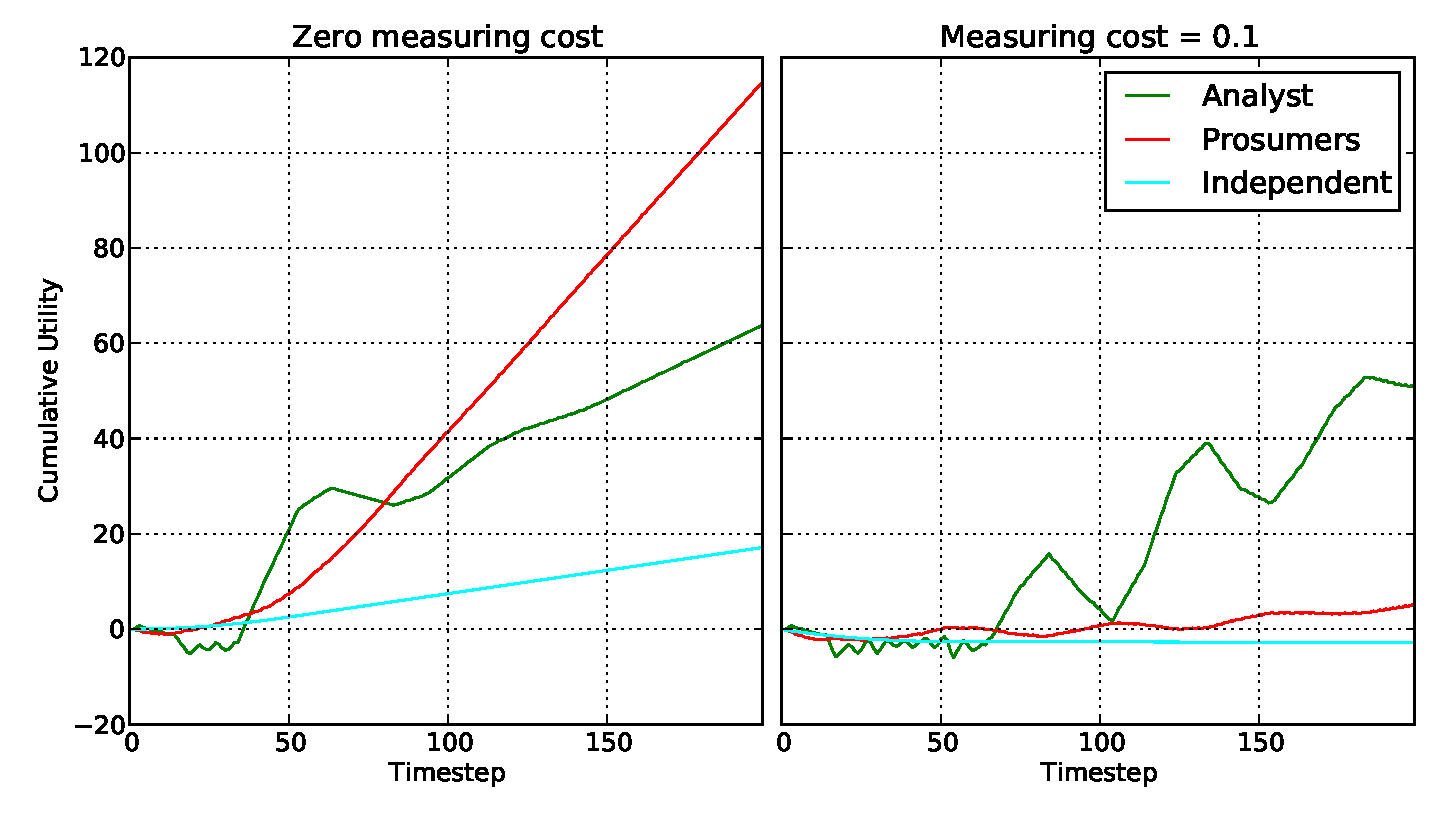
\includegraphics[width=\linewidth]{gfx/kc/market1.pdf} 
\caption{Cumulative utility of agent groups over time with a market, and zero and 0.1 measuring cost. Facility profile is high fixed.}\label{fig:market1}
\end{figure}

\subsubsection{Principled}

Under this governance scheme both analysts and prosumers can vote on appropriation rates for artifacts and a subscription fee for the institution. In order to prevent these votes being biased towards group, the ballot is weighted such that each group has an equal weighting across all its voters. Thus the vote represents a compromise across the preferences of the two groups.

Figure~\ref{fig:principled1} shows that this governance functions comparably to centralised in compensating agents.

\begin{figure}
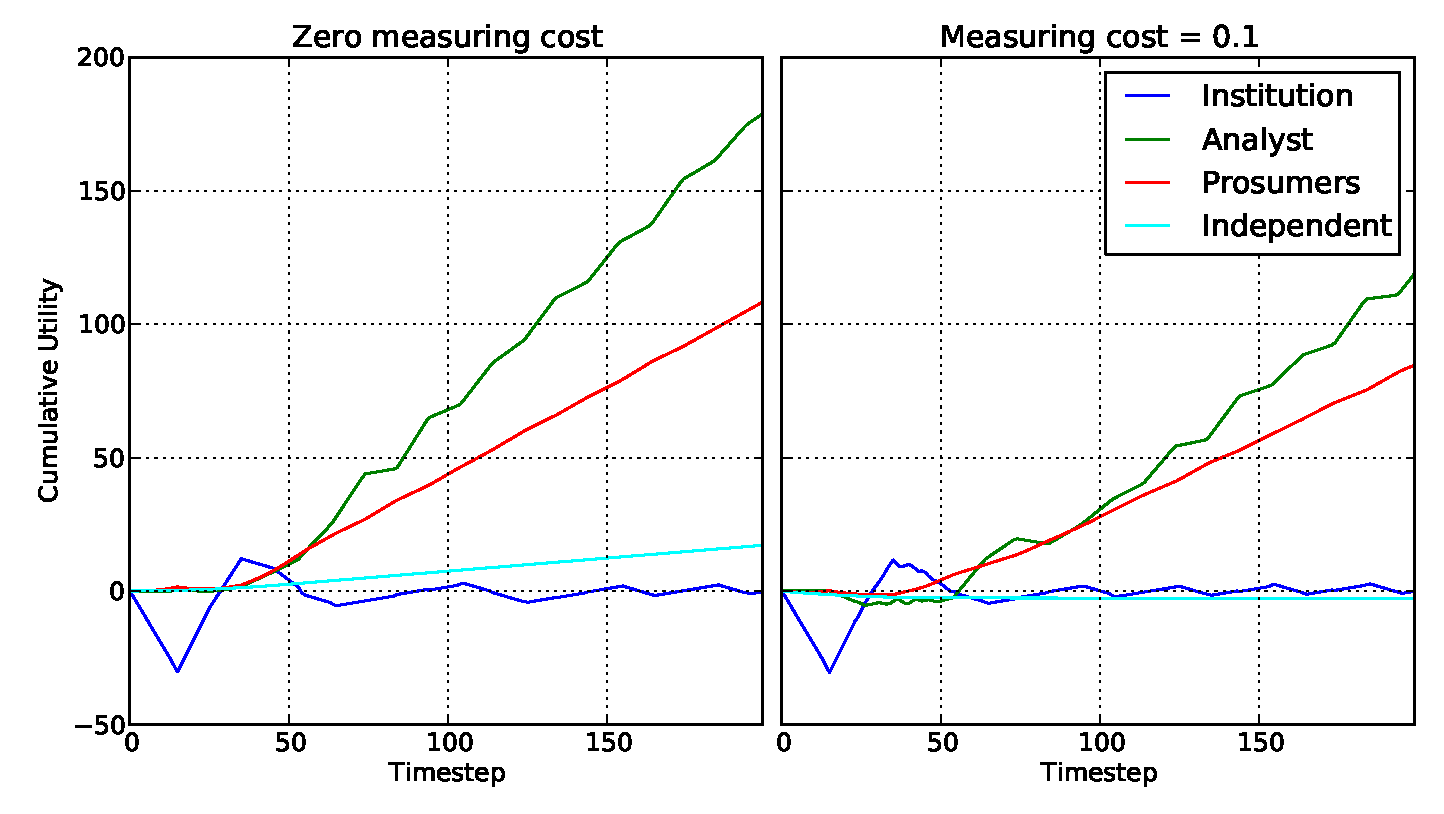
\includegraphics[width=\linewidth]{gfx/kc/principled.pdf} 
\caption{Cumulative utility of agent groups over time with collective governance according to Ostrom's third principle, and zero and 0.1 measuring cost. Facility profile is high fixed.}\label{fig:principled1}
\end{figure}

\subsection{Comparison of institutional paradigms}

We will not compare the three institutional paradigms with respect to the effect that malicious agent strategies can have on the institution.

\subsubsection{Individual Power}

How much difference can one agent changing strategy make? Figure~\ref{fig:powerbar} shows the difference in final utilities when individual agent strategies are changed to greedy ones. 

In a centralised regime only the initiator agent can affect the outcome, and he is able to extract significant utility for himself from the other participants. In the market-based case analysts are able to improve their score with more aggressive pricing, but prosumers are unable to benefit themselves - largely as too aggressive pricing causes the knowledge they appropriate to be worse. Finally, with principled governance no individual is able to benefit themselves, however a selfish majority of prosumers can significantly impact the analyst's utility.

\begin{figure}
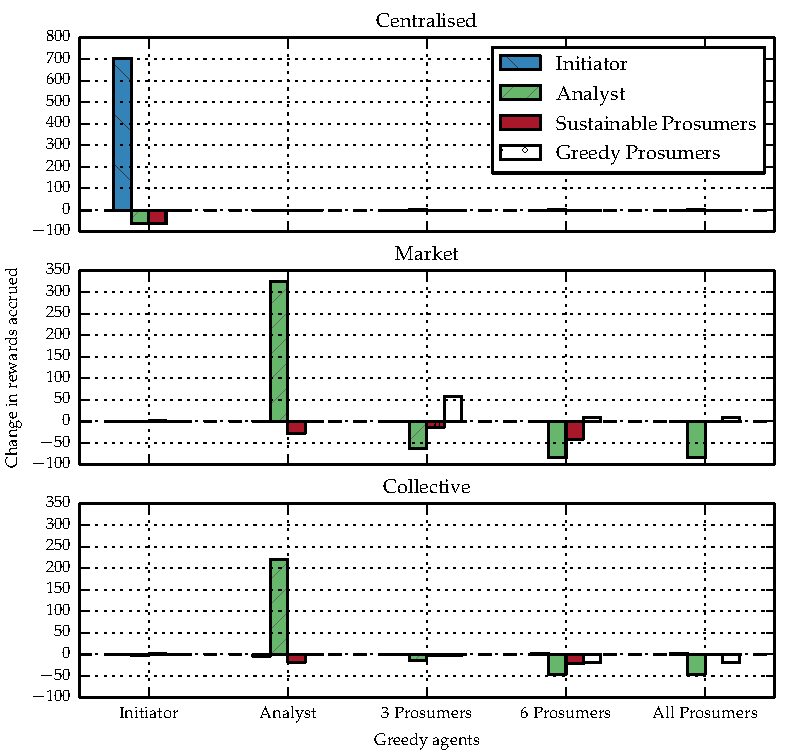
\includegraphics{gfx/kc/powerbar.pdf} 
\caption{Change in final utilities of agent groups when individuals change to a greedy strategy.}\label{fig:powerbar}
\end{figure}

From this we can conclude that both market and principled paradigms are much better at preventing self-interested individuals from exploiting the system, and also dis-incentivising non-cooperative behaviours.

\section{Evaluation \& Conclusions}

\begin{itemize}
\item The problem of supply: Institutions are hard to set-up, particularly early on.
\item Compensating desired roles: require self-organising mechanisms to incentivise desired behaviours.
\item Concentration of power: Too much power given to an individual can allow them to unfairly influence others' outcomes.
\item Centralised allows the \emph{initiator} agent to extract profit at will.
\item Market: price competition generally cancels out and also mostly prevents concentrated power. NC agents kept interested by compensation for provisions.
\item Collective: Robust to malicious agent strategies. Requires appropriate voting rules (weighted in this case).
\end{itemize}